\documentclass{article}
\usepackage{float}
\usepackage{graphicx}
\usepackage{hyperref}
\usepackage{geometry}
\geometry{left=2cm,right=2cm,top=2cm,bottom=2cm}

\begin{document}
\begin{itemize}
	\item Bayesian Market Paper:
	      \begin{itemize}
		      \item Question: $n$ buckets, what is the initial price so that the loss is bounded?
		      \item Utility Theory
		      \item Understand Bayesian form of the market maker.
	      \end{itemize}
	\item Exponential Family Market Paper:
	      \begin{itemize}
		      \item do not care too much about interpretation of the price meaning?
		      \item map log partition function with the Gaussian market (we did in the last week)
		      \item Equation $15$, slide in $EECS445$: prior distribution, update distribution: EM algorithm.
		      \item How informed you are as a trader (number of amount?): Kutty gives an example: A tosses the coin $5$ times, B tosses the coin $4$ times, C tosses the coin $6$ times, each of these correspond to how informed person A, B, C are about the true bias of the coin. (parameter $m$, $\hat{\mu}$, for each exponential family distribution, there is a prior in the general form, some for $m$ in $n$, $\mu$, in the agent case $\rightarrow$ conjugate prior: how much an agent knows about the true outcome).
		      \item market maker: current price $\rightarrow$ his belief. $m, \hat{\mu}$ corresponds to data.
		      \item TO DO: work this out for Gaussian market (Bayesian Market Paper).
	      \end{itemize}
	\item Agent shifting market example:
	      \begin{figure}[H]
		      \centering
		      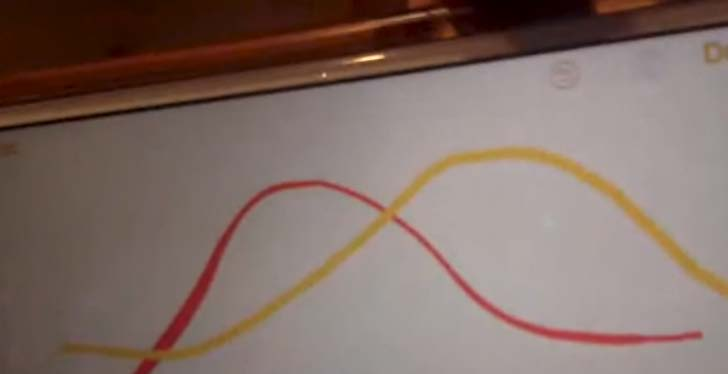
\includegraphics[scale=0.3]{./figure/before.jpg}
	      \end{figure}
	      Initial curve: red. An agent comes into the market: curve changes to green.
	      \begin{figure}[H]
		      \centering
		      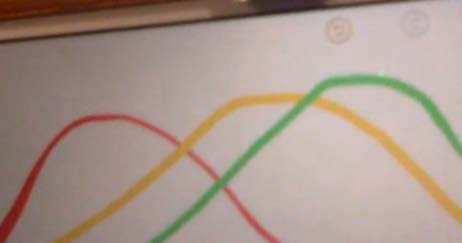
\includegraphics[scale=0.5]{./figure/after.jpg}
	      \end{figure}
	      Each agent's shifting corresponds to a data point. Data point number corresponds to how much the curve shifts. For instance, one trader has a hundred points, another with ten points, they would shift the curve differently.

	\item Market distribution and the curve distribution do not need to be from the same space.

	\item What is $x$, what is $\mu$? What is the connection between the shifting procedure and Posterior exception (what gets shifted, new $\nu$ value). Shifting $\nu$ based on data points. In reality, we do not know how many points agent has, but agent would shift the market state: trader has a strong belief in their data (because they might have access to other more date). Kutty gave an example: if one person flips a coin 5 times, with 4 heads and 1 tail. Agent knows it is biased, but he might suspect it is still unbiased. But if another agent flips it $10,000$ times, with $9000$ heads, then he might shift the probability distribution curve more in favor of bias.
	\item Current market state: prior understanding. Agent comes in $\rightarrow$ update of understanding. (Kutty suggested we might think in the case of Gaussian distribution)
	\item Kutty said in the future, we might simulate manipulation of the prediction market. She likes the idea of spread, she said we could do simulation on loss being function of a spread.

	\item Send email on Thursday about Yiling's paper: interpret market (the equation: midpoint? spread?). Search: what is the meaning of that equation?
	\item Next Thursday: presentation about repetition project checkpoint. (might be recorded)
	\item Initial goal: Gaussian Bernoulli, corresponding conjugate prior for Bayesian Market Maker from exponential family market maker section $4$ (implementation). Exponential Family Market 5.2. Exponential utility, utility function meaning (tied to Bayesian Market). Do not worry about Game Theory. Re-derive the Gaussian for 5.2 section.
	\item Paper talks about convergence rate:\href{https://www.cs.colorado.edu/~raf/media/papers/risknets.pdf}{Convergence rate paper} different context. This might be a research project later.
\end{itemize}
\end{document}
